%%%%%%%%%%%%%%%%%%%%%%%%%%%%%%%%%%%%%%%%%
% Short Sectioned Assignment
% LaTeX Template
% Version 1.0 (5/5/12)
%
% This template has been downloaded from:
% http://www.LaTeXTemplates.com
%
% Original author:
% Frits Wenneker (http://www.howtotex.com)
%
% License:
% CC BY-NC-SA 3.0 (http://creativecommons.org/licenses/by-nc-sa/3.0/)
%
%%%%%%%%%%%%%%%%%%%%%%%%%%%%%%%%%%%%%%%%%

%----------------------------------------------------------------------------------------
%	PACKAGES AND OTHER DOCUMENT CONFIGURATIONS
%----------------------------------------------------------------------------------------

\documentclass[paper=a4, fontsize=11pt]{scrartcl} % A4 paper and 11pt font size

\usepackage[T1]{fontenc} % Use 8-bit encoding that has 256 glyphs
\usepackage{fourier} % Use the Adobe Utopia font for the document - comment this line to return to the LaTeX default
\usepackage[english]{babel} % English language/hyphenation
\usepackage{amsmath,amsfonts,amsthm} % Math packages

\usepackage{sectsty} % Allows customizing section commands
\allsectionsfont{\centering \normalfont\scshape} % Make all sections centered, the default font and small caps

\usepackage{fancyhdr} % Custom headers and footers
\pagestyle{fancyplain} % Makes all pages in the document conform to the custom headers and footers
\fancyhead{} % No page header - if you want one, create it in the same way as the footers below
\fancyfoot[L]{} % Empty left footer
\fancyfoot[C]{} % Empty center footer
\fancyfoot[R]{\thepage} % Page numbering for right footer
\renewcommand{\headrulewidth}{0pt} % Remove header underlines
\renewcommand{\footrulewidth}{0pt} % Remove footer underlines
\setlength{\headheight}{13.6pt} % Customize the height of the header

\numberwithin{equation}{section} % Number equations within sections (i.e. 1.1, 1.2, 2.1, 2.2 instead of 1, 2, 3, 4)
\numberwithin{figure}{section} % Number figures within sections (i.e. 1.1, 1.2, 2.1, 2.2 instead of 1, 2, 3, 4)
\numberwithin{table}{section} % Number tables within sections (i.e. 1.1, 1.2, 2.1, 2.2 instead of 1, 2, 3, 4)

\setlength\parindent{0pt} % Removes all indentation from paragraphs - comment this line for an assignment with lots of text

% JK custom setup
\usepackage[noabbrev]{cleveref}
\usepackage{hyperref}
\usepackage{graphicx}
% end JK custom setup

%----------------------------------------------------------------------------------------
%	TITLE SECTION
%----------------------------------------------------------------------------------------

\newcommand{\horrule}[1]{\rule{\linewidth}{#1}} % Create horizontal rule command with 1 argument of height

\title{	
\normalfont \normalsize 
\textsc{University of Paderborn} \\ [25pt] % Your university, school and/or department name(s)
\horrule{0.5pt} \\[0.4cm] % Thin top horizontal rule
\huge Usability Test -- Implicit Feedback Analysis System \\ % The assignment title
\horrule{2pt} \\[0.5cm] % Thick bottom horizontal rule
}

\author{Janis Krasemann} % Your name

\date{\normalsize\today} % Today's date or a custom date

\begin{document}

\maketitle % Print the title

%----------------------------------------------------------------------------------------
%	Usability Test
%----------------------------------------------------------------------------------------

You are asked to do a usability test on a customized version of the Mattermost chat application.
[Blabla about usability testing...]
Please try to execute the tasks as precisely as possible.
Just do the tasks to the best of your ability, your performance will not be graded in any kind.
Some of your actions will be automatically recorded via the implicit user feedback analysis system, the data is completely anonymous though.
In fact, you do not even have to input any personal information -- instead, a username and password is already prepared for you and printed in \ref{task0}.

%------------------------------------------------

\section{Login}
\label{task0}

Using a web browser that you are familiar with, such as Google Chrome, Firefox, or Safari, navigate to \url{http://localhost}.
You will be presented a login screen in which you can input the following login information:

\begin{itemize}
\item Username: jibem
\item Password: 12345678
\end{itemize}

\textbf{Important:} Please check whether you are shown a blue menu at the left side of the screen -- if not, please increase the size of your browser window until the menu apperas (cf. the screenshot in figure \ref{menu-example}).

Click the button labeled "Sign in", then proceed to \ref{task1}.

\begin{figure}[htb]
        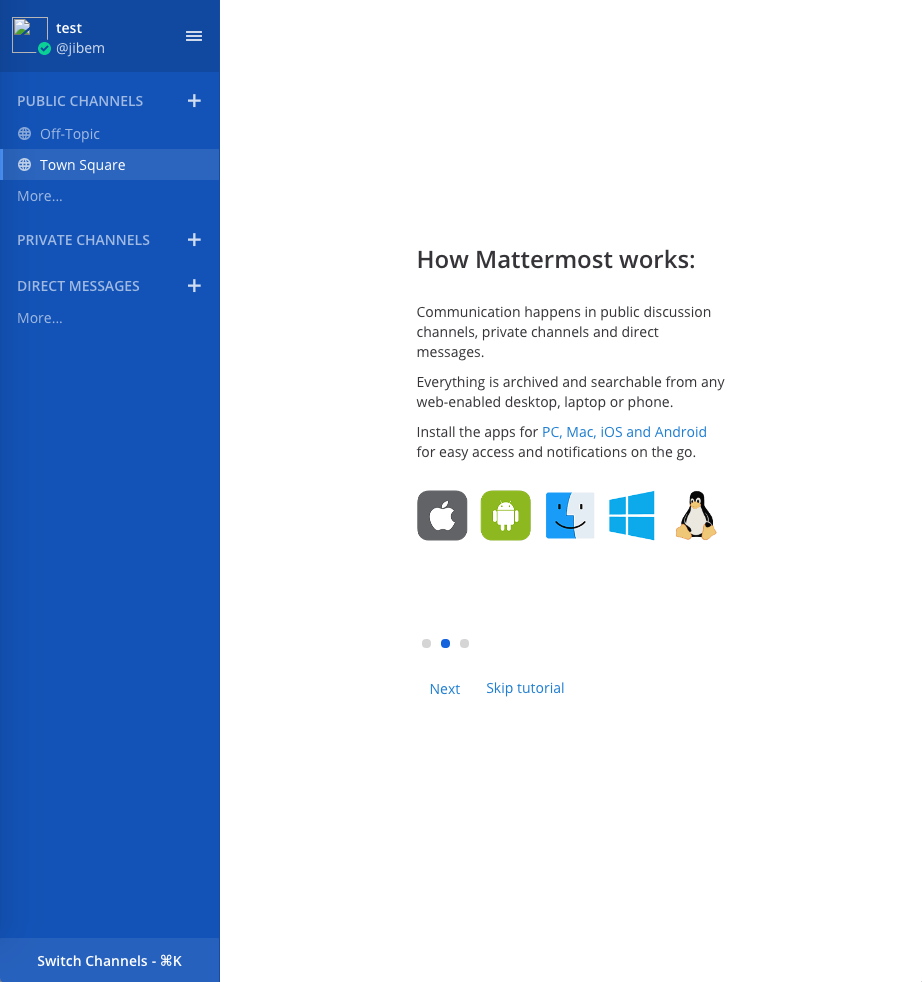
\includegraphics[width=\textwidth]{menu-example}
        \caption{If needed, resize your browser window such that the blue side menu appears. TODO: Update}
        \label{menu-example}
\end{figure}


%------------------------------------------------

\section{Tutorial}
\label{task1}

If you have not yet used a web based chat application, or otherwise think you need a short introduction to Mattermost, feel free to go through the tutorial.

\textbf{Assignment}:If you want to do the tutorial, feel free to read the introductory text in the center of the screen, then click the button labeled "Next".
If you do not want to do the tutorial, click the link labeled "Skip tutorial".

When you have done this and are shown a number of cat pictures (because you are in the "Cats" channel initially), you can proceed to \ref{task2}

%------------------------------------------------

\section{Channel Switching}
\label{task2}

In the menu on the left side of the screen, you can see a list of "public channels".
Channels are chat groups that you can join in order to write and read messages there.
There are currently only two public channels: "Cats" and "Dogs".
You are currently in the Cats channel.

\textbf{Assignment}: Click the entry for the Dog channel in the menu on the left side of the screen in order to change to this channel.
If the main window's contents change to some dog pictures, you have succeeded.

\subsection{Using the Channel Switcher}

There is another possibility for switching channels, called the "Channel Switcher".
You can bring up the channel switcher by either clicking the "Switch Channels" button at the bottom left corner of the window, or by pressing Ctrl+K / Cmd+K (depending on whether you use a Windows or Mac computer).
In the channel switcher, you can switch between channels by typing (part of) the name of the desired channel and then clicking the channel that you want to switch to.

\textbf{Assignment}: Bring up the channel switcher by clicking the "Switch Channels" button, then type "Cats" and click the appearing entry for the "Cats" channel.
If you are again shown various cat pictures, you have succeeded.

\subsection{Switch channels one more time}

\textbf{Assignment}: As dogs are obviously superior, you now want to change back to the Dogs channel.
Please do so either via the channel switcher on the bottom left corner, or by clicking the channel directly in the menu on the left side of the screen -- it's up to you.

When you have done this, please continue to the final task \ref{task4}.

%------------------------------------------------

\section{Send a message}
\label{task4}

Of course, Mattermost also offers the possibility for users to write messages in any channel that they are part of.
This is done by clicking into the text box at the bottom of the window, then writing the message and finally hitting the enter key.

\textbf{Assignment}: Write a message into the text box at the bottom of the window, then press the enter key to send it.
The contents of the message are up to you, it can just be a simple "hello" or something more elaborate.

%------------------------------------------------

\section{Wrap-up}
\label{wrapup}

???

%----------------------------------------------------------------------------------------
%	PROBLEM 2
%----------------------------------------------------------------------------------------
%
%\section{Lists}
%
%%------------------------------------------------
%
%\subsection{Example of list (3*itemize)}
%\begin{itemize}
%	\item First item in a list 
%		\begin{itemize}
%		\item First item in a list 
%			\begin{itemize}
%			\item First item in a list 
%			\item Second item in a list 
%			\end{itemize}
%		\item Second item in a list 
%		\end{itemize}
%	\item Second item in a list 
%\end{itemize}
%
%%------------------------------------------------
%
%\subsection{Example of list (enumerate)}
%\begin{enumerate}
%\item First item in a list 
%\item Second item in a list 
%\item Third item in a list
%\end{enumerate}

%----------------------------------------------------------------------------------------

\end{document}